\documentclass[12pt,twoside]{article}

\usepackage[T1]{fontenc}
\usepackage[utf8]{inputenc}
\usepackage[spanish]{babel}

\let\layoutspanish\relax
\addto\captionsspanish{\def\tablename{Tabla}}
\unaccentedoperators

\usepackage[a4paper]{geometry}
  \geometry{hmargin={2.5cm,2.5cm},height=22cm}
  
\renewcommand{\baselinestretch}{1.2}  
\setlength{\partopsep}{0pt}
\setlength{\itemsep}{0pt}
\setlength{\topsep}{0pt}
\setlength{\parsep}{0pt}
\setlength{\parskip}{0.25\baselineskip}

\renewcommand{\textfraction}{0.1}
\renewcommand{\topfraction}{1}
\renewcommand{\bottomfraction}{1}
\renewcommand{\floatpagefraction}{1}

\setcounter{totalnumber}{5}
\setcounter{topnumber}{3}
\setcounter{bottomnumber}{2}

\usepackage{caption}


\usepackage{indentfirst}

\usepackage[pdftex]{color}

\usepackage[pdftex]{graphicx}

\usepackage{amsmath}
\allowdisplaybreaks 
\usepackage{amssymb}
\usepackage{amsfonts} 
\usepackage{enumerate}

\usepackage{fancyhdr}

\newcommand{\RunningAuthor}{Ginés Meca Carbonell}
\newcommand{\Author}[1]{\renewcommand{\RunningAuthor}{#1}}
\renewcommand{\leftmark}{\RunningAuthor}

\newcommand{\RunningTitle}{Métodos de Machine Learning basados en Árboles de Decisión.}
\newcommand{\Title}[1]{\renewcommand{\RunningTitle}{#1}}
\renewcommand{\rightmark}{\RunningTitle}

\pagestyle{fancy}
\fancyhf{}
\fancyhead[LO]{\small \slshape \leftmark}    
\fancyhead[RE]{\small \slshape \rightmark}   
\fancyhead[RO,LE]{\small \slshape \thepage}  

\renewcommand{\headrulewidth}{0.6pt}         
\renewcommand{\footrulewidth}{0pt}           
                                             
\setlength{\headheight}{1.5\headheight}      

\fancypagestyle{plain}{%                     
  \fancyhf{}                                 
  \setlength{\headwidth}{\textwidth}
  \fancyfoot[C]{\small \slshape \thepage}    
  \renewcommand{\headrulewidth}{0pt}
  \renewcommand{\footrulewidth}{0pt}
  }
  
\newcommand{\abs}[1]{\ensuremath{|#1|}}

\usepackage{hyperref}

\title{Métodos de Machine Learning basados en Árboles de Decisión}
\author{Ginés Meca Carbonell\\*[1em]
\begin{minipage}{0.75\textwidth}
\footnotesize \itshape
\begin{center}
Universidad de Alicante \\
4º de Grado en Matemáticas
\end{center}
\end{minipage}
}
\date{Junio 2022}

\usepackage{pdfpages}




\begin{document}


\includepdf[pages=1]{anexo-1-portada-memoria-tfg-matematicas.pdf}



\section*{Resumen}

\emph{En este trabajo, se ha estudiado el conjunto de algoritmos de Machine Learning derivados de los árboles de decisión.}

\newpage



\section*{Abstract}

\emph{}

\newpage



\tableofcontents



\newpage



\section{Introducción}

Vivimos en la era de la información. Cada segundo, millones de datos viajan entre diferentes lugares del planeta y se guardan formando enormes conjuntos de datos. Además, cada vez hay más instrumentos capaces de recoger información. Donde antes se necesitaba hacer uso de encuestas, ahora nos encontramos con dispositivos, como los teléfonos móviles, capaces de escribir texto, recoger audio y realizar fotografías y vídeos. Así, la información a nuestra alcance es infinita. Podemos conocer cuáles son los conceptos que son tendencia en los buscadores de internet, o cuáles son aquellos audiovisuales que más éxito están teniendo en las redes sociales. Del mismo modo, podemos acceder al historial de imágenes de la cámara de seguridad de nuestra vivienda o a la tabla que recoge las últimas operaciones de nuestra empresa. Es fácil obtener grandes cantidades de datos de aquello que nos interesa.

Dado que el número de datos que manipulamos cada vez es mayor,las técnicas utilizadas para analizarlos van evolucionando constantemente. Muchas de las técnicas clásicas del análisis de datos han quedado obsoletas, otras se utilizan para crear algoritmos más complejos. Uno de los algoritmos más conocidos es el de los árboles de decisión. Fueron introducidos por primera vez en 1963 por James N. Morgan y John A. Sonquist, quienes obtuvieron un método muy eficaz a través de un algoritmo muy básico. Actualmente, existen diferentes algoritmos que se pueden emplear a la hora de generar un árbol de decisión: CHAID, C4.5, FACT, QUEST, CRUISE... No obstante, el más conocido, y el que estudiaremos en este trabajo, es el algoritmo CART (Classification And Regression Trees), creado por Breiman, Friedman, Olshen y Stone en 1984. De hecho, fue el propio Leo Breiman quien, basándose en CART, desarrolló años más tarde el algoritmo Random Forest. Paralelamente, la publicación de Freund y Schapire en 1997 de un nuevo método basado en boosting daría lugar a otra serie de algoritmos; es aquí donde nos encontramos algoritmos más complejos, como el xgboost, que ocuparán gran parte del trabajo.

Dado que en los últimos años varios alumnos han realizado su TFG sobre árboles de decisión explicando su estructura más básica, resumiré las secciones dedicadas a ello con el fin de centrarme en analizar a fondo los algoritmos más complejos y novedosos que no se han tratado en estos trabajos y, así, elaborar un mapa conceptual de modelos lo más completo posible.



\subsection{Datos: Llueve en Australia} \label{sec: subsec11}

Para hacernos una idea de cómo funciona cada uno de los algoritmos detallados a lo largo del trabajo, haremos uso del conjunto de datos indicado. Se trata de un dataset en el que podemos encontrar mediciones de diferentes variables meteorológicas así como la fecha y localidad correspondientes y la información relativa a si llovió o no el día de la medición y el día siguiente.
\begin{figure}[h]
	\centering
	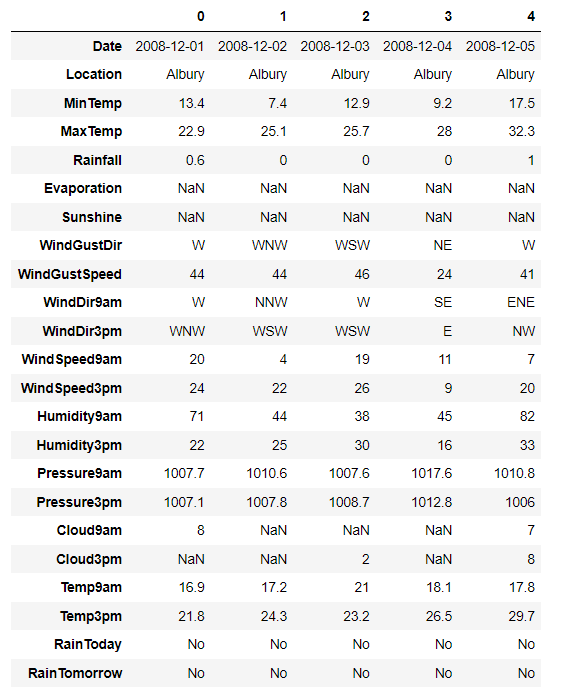
\includegraphics[width = 0.4\textwidth]{Intro_01}
	\caption{Encabezado del dataset}
\end{figure}

En total, se tiene 23 columnas que recogen información de 145460 días.


\subsection{Metodología}

A la hora de aplicar los diferentes métodos al conjunto de datos se procederá mediante validación cruzada. Es decir:

\begin{enumerate}
\item Se selecciona el modelo correspondiente.
\item Se separa, al azar, el conjunto de datos inicial en dos: datos de entrenamiento y datos de testeo.
\item Se entrena el modelo con los datos de entrenamiento.
\item Se aplica el modelo entrenado a los datos de testeo.
\item Se comprueba la veracidad de las predicciones realizadas.
\end{enumerate}

Habitualmente, la división del conjunto inicial que da lugar a los subconjuntos de entrenamiento y testeo se realiza de manera aleatoria. No obstante, dada la naturaleza de los datos, procederemos de otra manera.

Separando el conjunto de datos de manera aleatoria nos encontraremos con que los datos de testeo se encontrarán intercalados con los de entrenamiento. Esto puede ocasionar que la predicción de testeo a realizar se encuentre entre dos datos utilizados al entrenar el modelo. Este método no es erróneo, pero no nos da ninguna información acerca de cómo se desenvuelve el algoritmo a la hora de clasificar datos de fechas posteriores.

Entonces, el procedimiento será ligeramente distinto, emplearemos la validación 'Out Of Time'. Dado que nuestro dataset contiene fechas desde el 01/11/2007 hasta el 24/06/2017, nuestro conjunto de entrenamiento estará formado por todos aquellos datos con fecha anterior al 01/01/2015 y los datos de testeo serán los restantes. Así, entrenamos el modelo con datos anteriores a los de testeo para saber cómo van a ser las predicciones futuras y asemejarnos más a lo que nos interesaría en un caso real: entrenar el modelo de manera que al introducir las fechas actuales, no registradas, y de las cuales no sabemos que ocurrirá unos días o semanas más tarde en función de los datos que poseemos sobre fechas posteriores.

Además, los cálculos se realizarán en el lenguaje de programación Python. Todo el código se encuentra disponible en el Anexo (\ref{sec:Anexo}).



\newpage



\section{Árboles de decisión CART}
\subsection{Preliminares}

Los árboles de decisión son muy utilizados como método predictor (tanto de regresión como de clasificación) dada su simpleza, su efectividad y lo visual que resulta su funcionamiento a través de un gráfico, lo cual facilita su comprensión. Se trata de un algoritmo que divide sucesivamente el conjunto inicial de datos en diferentes subconjuntos a través de diversas condiciones relacionadas con sus variables explicativas. Por ejemplo:

\textbf{Ejemplo 2.1: } \textit{Se pretende estudiar la variable 'RainTomorrow' del conjunto de datos dado en función de las variables explicativas 'Cloud3pm' y 'Humidity3pm'(nivel de nubosidad y de humedad a las 15.00, respectivamente) para predecir si lloverá o no al día siguiente. Así, escogiendo únicamente las variables explicativas indicadas, el esquema que seguirá nuestro árbol de clasificación será el siguiente: }
\begin{figure}[h]
	\centering
	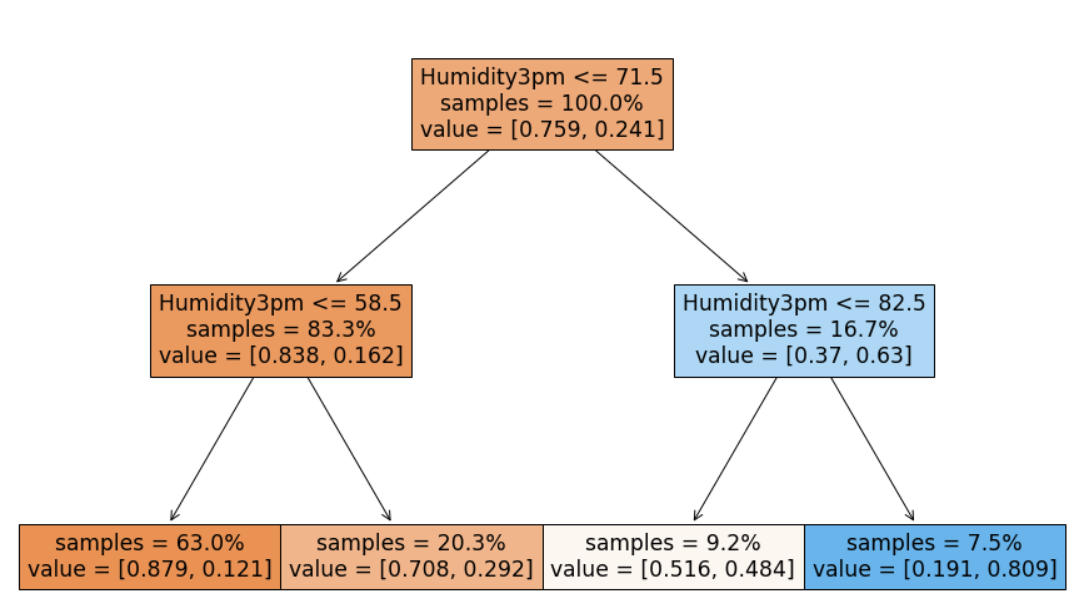
\includegraphics[width = 0.7\textwidth]{ex2_1_01}
	\caption{Ejemplo 2.1. Árbol de decisión}
	\label{fig:Ejemplo 2.1}
\end{figure}

Como se puede observar, el algoritmo es muy intuitivo: se introduce un individuo y se le aplica la primera condición; si la respuesta es afirmativa se sigue el camino de la izquierda y si es negativa el de la derecha. Mediante este proceso, se va comprobando si sus variables explicativas cumplen las diferentes condiciones que se plantean hasta llegar a un grupo que deja de dividirse, que será su predicción.

Por otro lado, es fácil ver que las condiciones del algoritmo se corresponden con particiones del espacio. Como en el ejemplo anterior se han elegido únicamente dos variables explicativas, se puede hacer una representación de los individuos sobre $\mathbb{R}^{2}$ y determinar sobre él las diferentes regiones de predicción.
\begin{figure}[h]
	\centering
	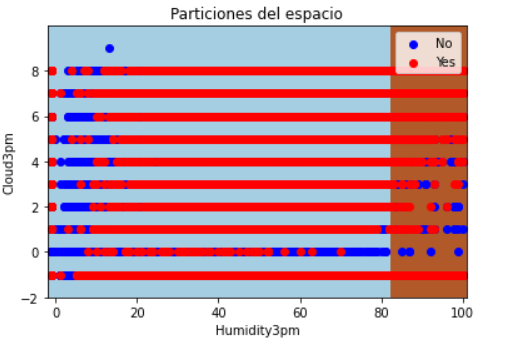
\includegraphics[width = 0.5\textwidth]{ex2_1_02}
	\caption{Partición del espacio del Ejemplo 2.1}
	\label{fig:Ejemplo 2.1.2}
\end{figure}


\subsubsection{Notación y conceptos básicos}

A continuación, se introducirán una serie de términos básicos para poder hacer referencias correctas a los conceptos presentados. Por un lado, nos encontramos con las siguientes definiciones:
\begin{description}
\item[Nodo raíz: ]Primer nodo, que contiene a todos los individuos, a partir del cual comienzan a realizarse las divisiones.
\item[Nodo interno: ]Nodos intermedios que provienen de una división y desencadenan otra. Dentro de ellos, se pueden definir:
	\begin{description}
	\item[Nodo padre: ]Nodo anterior a un nodo interno fijado.
	\item[Nodos hijos: ]Nodos resultantes de la división del nodo interno fijado.
	\end{description}
\item[Nodo hoja: ]Nodos finales que dan lugar a la predicción.
\end{description}

Se pueden identificar todos estos nodos en la figura del ejemplo 2.1 (\ref{fig:Ejemplo 2.1}). Se tienen un nodo raíz, seis nodos internos y 8 nodos hoja.

Por otro lado, conviene hablar del concepto de sobreajuste (en inglés: overfitting). Se dice que un modelo se encuentra sobreajustado si el algoritmo se ha adaptado en exceso a los individuos del conjunto de entrenamiento. Este hecho provoca que la predicción de los individuos de este conjunto sea muy buena, mientras que al introducir nuevos individuos estas predicciones presentan grandes errores.

Para lidiar con el sobreajuste, interesa manejar también otras dos nociones: el sesgo y la varianza. El sesgo (en inglés: bias) hace referencia a los errores cometidos en las predicciones de los individuos de nuestro conjunto de entrenamiento. Por contra, la varianza es la medida del error cometido en los individuos que no pertenecen a este conjunto; en nuestro caso, lo mediremos en los individuos del conjunto de testeo. No obstante, estos conceptos generan un problema: interesa tener valores bajos de ambos indicadores, pero disminuir el sesgo conlleva un aumento de la varianza. Así, a la hora de construir un modelo de Machine Learning, interesa estudiar que el sesgo no sea excesivamente bajo, para evitar el sobreajuste, pero también que no sea excesivamente alto para que las predicciones sean fiables.


\subsubsection{Objetos de estudio de un CART}

Una vez visto cómo se realizan las predicciones al trabajar con árboles de decisión, corresponde explicar el funcionamiento del mismo. Para ello, habrá que tratar los siguientes aspectos:
\begin{enumerate}
\item Elección de variables y valores asociados a cada nodo interno.
\item Criterio de parada de división de los nodos
\item Valor o clase asignada a cada nodo
\end{enumerate}


\subsection{Elección de variables y valores asociados a cada nodo interno} \label{sec: subsec22}
Sea un conjunto de datos de n individuos y p+1 variables ($n,p \in \mathbb{N}$). De este modo, sean $X_1, X_2, ... , X_p$ las variables explicativas e $y$ la variable dependiente. En el caso de nuestro conjunto de datos de ejemplo:
\begin{table}[h]
\centering
\begin{tabular}{rcccc|c}
 & \multicolumn{1}{l}{$X_1$}         & $X_2$                        & ...                      & $X_{22}$ & $y$ \\ \hline
\multicolumn{1}{l|}{$x_1$} & \multicolumn{1}{r|}{2008-12-01} & \multicolumn{1}{l|}{Albury} & \multicolumn{1}{l|}{...} & No        & \multicolumn{1}{l|}{No} \\ \hline
\multicolumn{1}{l|}{$x_2$} & \multicolumn{1}{r|}{2008-12-02} & \multicolumn{1}{l|}{Albury} & \multicolumn{1}{l|}{...} & No        & \multicolumn{1}{l|}{No} \\ \hline
\multicolumn{1}{l|}{$x_3$} & \multicolumn{1}{r|}{2008-12-03} & \multicolumn{1}{l|}{Albury} & \multicolumn{1}{l|}{...} & No        & \multicolumn{1}{l|}{No} \\ \hline
\end{tabular}
\end{table}

Pese a las similitudes existentes entre los árboles de regresión y los de clasificación, conviene dividir este apartado en dos con tal de mostrar el funcionamiento exacto de cada uno de ellos.


\subsubsection{Árboles de regresión}
Se busca conocer cómo realizar las divisiones. En particular, nos centraremos en la primera división y el proceso será similar para las siguientes. Al situarnos en el nodo raíz, nos encontramos con el conjunto de datos al completo y pretendemos dividirlo en dos regiones, que denotaremos $R_1$ y $R_2$, en función de una de las variables explicativas, $X_j$, y de un valor respecto de esta, s, de manera que:
\begin{equation*}
R_1 (j,s) = \{ X | X_j \leq s \} \, \, \, \wedge \, \, \,  R_2 (j,s) = \{ X | X_j > s\}
\end{equation*}

Sabemos que $Y_1$ se mantendrá constante sobre $R_1$ y que $Y_2$ también será constante sobre $R_2$. De esta manera, buscamos j y s tales que:
\begin{equation*}
\min_{j,s}(\min_{c_1, c_2}(\sum_{x_i \in R_1}(y_i - c_1)^2 + \sum_{x_i \in R_2}(y_i - c_2)^2))
\end{equation*}
o lo que es lo mismo, buscamos j y s que minimicen el error cometido en la predicción de los individuos del conjunto de entrenamiento. Esta tarea se puede llevar a cabo probando todos los casos posibles y escogiendo el que minimice la expresión.


\subsubsection{Árboles de clasificación}
En el caso de los árboles de clasificación, la variable dependiente es una clase; es decir, como en la tabla dada al comienzo de la subsección (\ref{sec: subsec22}). Ahora, en lugar del error mínimo cuadrático, introduciremos una función de impureza que nos permita evaluar la homogeneidad de los nodos; es decir, que nos permita estudiar qué acciones separan mejor el espacio en función de las diferentes clases. El criterio más empleado es el índice Gini, que se define como:
\begin{equation*}
G_{region} = \sum_{k=1}^K p_{mk}(1 - p_{mk})
\end{equation*}
donde $p_{mk}$ es la proporción de individuos del conjunto de entrenamiento de clase k que se encuentran en la región m y K es el número total de clases. Así, fijado un m, se puede calcular el índice Gini de una determinada región. Además, se puede observar que valores de $p_{mk}$ cercanos a 0 o 1 implican que el producto $p_{mk}(1- p_{mk})$ sea muy pequeño. Por tanto, el índice Gini actúa como medidor de la pureza de una región: un índice Gini bajo significa que los diferentes $p_{mk}$ están cercanos a 0 o 1 y la región es "pura".

Sabiendo esto, solo queda evaluar el índice Gini de un nodo. Esto se hace mediante una media ponderada, es decir:
\begin{equation*}
G_{nodo} = \frac{n_1}{n_1 + n_2}G_1 + \frac{n_2}{n_1 + n_2}G_2
\end{equation*}
donde  $n_1$ y $n_2$ son la cantidad de individuos de las regiones $R_1$ y $R_2$, respectivamente, y $G_1$ y $G_2$ son los índices Gini de las mismas. Así, la tarea se resume en obtener, mediante comprobación de todas las opciones posibles, la variable y el valor que minimizan el índice Gini del nodo.




\subsection{Criterio de parada de escisión de nodos}
Se podría pensar que la precisión de un CART aumenta conforme aumenta en profundidad, es decir, conforme aumenta en número de particiones. No obstante, como ya se ha introducido, cuantas más particiones del espacio realice el algoritmo, más se estará ajustando a los datos del conjunto de entrenamiento, lo que puede llevar a sobreajuste. Con tal de evitar este hecho, se han implementado algunos métodos de "poda" del árbol. Es evidente que podando el árbol se introduce sesgo, pues no dejamos que se adecue totalmente a los datos de entrenamiento; sin embargo, haciendo esto de manera controlada se consigue disminuir la varianza y mejorar las predicciones.

Por un lado, la técnica más simple consiste en establecer una profundidad máxima. Con esta condición, se puede asegurar que los nodos dejarán de dividirse una vez alcanzado el nivel indicado. Por ejemplo, en el Ejemplo 2.1 (Figura \ref{fig:Ejemplo 2.1}) se ha establecido una profundidad máxima igual a 3.

Por otro lado, el árbol determinará un nodo como nodo hoja cuando la separación del mismo no sea conveniente en términos de pureza. El procedimiento es el siguiente: en primer lugar, se calcula el índice Gini de la región asociada a ese nodo y, después, se realiza la división del nodo y se calcula el índice Gini del mismo(proveniente de la media ponderada de índices de sus regiones). Si el índice de la región sin dividir es inferior al índice del nodo, se deshará la división y se determinará el nodo como nodo hoja, pues de esta manera se mantiene una mayor pureza.


\subsection{Valor o clase asignada a cada nodo hoja} \label{sec:2.4}
Como se comentaba anteriormente, el resultado de un árbol de decisión es una partición del espacio. Supongamos que se obtienen M regiones diferentes denotadas por $R_{m}$ con $m = 1, ..., M$. Por tanto, definamos como Y al árbol de decisión y como $c_m$, con $m = 1,...,M$, a las predicciones (imágenes de Y) asociadas a cada región $R_m$. De este modo:
\begin{equation*}
Y(x) = \sum^M_{m = 1} c_{m}I(x \in R_m) \, \, \, \forall x \in D
\end{equation*}
donde D es el dominio de la función (espacio de las variables explicativas) e I es la función indicadora:
\begin{equation*}
I(x) = 
\left.
\begin{array}{ccc}
1 & si & x \in R_m \\
0 & si & x \not\in R_m 
\end{array}
\right\}
\end{equation*}


Así, a la hora de entrenar un modelo, se busca minimizar los errores entre y e Y. Por ejemplo, si tomamos el error mínimo cuadrático, llegamos al problema:
\begin{equation*}
\min_{Y_i} \sum_{i=1}^n (y_i - Y_i)^2 \Rightarrow \min_{c_m} \sum_{m = 1}^M \sum_{x_i \in R_m} (y_i - c_m)^2
\end{equation*}
donde $Y_i = Y(x_i) \, \, \forall i=1,...n$. Si denotamos $f(c_m) = \sum_{x_i \in R_m} (y_i - c_m)^2$, observamos que alcanzar la solución óptima del problema planteado es equivalente a minimizar la función f:
\begin{equation*}
f'(c_m) = -2 \sum_{x_i \in R_m} (y_i - c_m) = -2 \sum_{x_i \in R_m}y_i + 2n_mc_m = 0 \Leftrightarrow c_m = \frac{1}{n_m} \sum_{x_i \in R_m}y_i
\end{equation*}
y
\begin{equation*}
f''(c_m) = -2 \sum_{x_i \in R_m} (-1) = 2n_m > 0
\end{equation*}
donde $n_m$ es el conjunto de datos pertenecientes a la región $R_m$, $\forall m = 1,...M$.

En conclusión, el valor asignado a cada nodo hoja será la media de las observaciones de los individuos del conjunto de entrenamiento que pertenecen a dicho nodo.

En el caso de árboles de clasificación, la tarea se simplifica: basta con calcular la proporción de individuos de cada clase en cada región y, así, el valor asignado a cada subconjunto del espacio será la clase a la que le corresponde la mayor proporción en el mismo.


\subsection{Ejemplo}
\textit{Se desea obtener una predicción fiable acerca de las precipitaciones del día siguiente en una ciudad de Australia. Para ello, haciendo uso del dataset anteriormente introducido, se dividirá el conjunto de datos en dos subconjuntos: uno de entrenamiento y otro de testeo. Además, probaremos con diferentes profundidades máximas permitidas para así construir el árbol más fiable.}

\textit{Además, con tal de analizar los resultados, utilizaremos el AUC; es decir, el área bajo la curva ROC('Area Under the Curve'), creada en base a la sensibilidad(tasa de  verdaderos positivos) y especifidad(tasa de verdaderos negativos) de las predicciones. Así, operando el AUC de la forma $2 \times AUC - 1$ obtenemos el coeficiente Gini(no confundir con el índice Gini de escisión de nodos). Cuanto más alto sea el valor de este coeficiente, mejor será nuestro clasificador.}

\textit{Con esto, aplicando los diferentes árboles de clasificación, llegamos al siguiente resultado:}

\begin{figure}[h]
\centering
\includegraphics[width = 0.3\textwidth]{ex2_2_01}
\caption{Resultados árboles de clasificación para RainTomorrow}
\end{figure}

\textit{En la tabla se ven reflejados los coeficientes de Gini para los conjuntos de entrenamiento y testeo y el porcentaje de información que se pierde en el conjunto de testeo respecto del de entrenamiento.}

\textit{Como podemos observar, cuando la profundidad máxima permitida es superior o igual a 10, el modelo empieza a sobreajustarse a los datos de entrenamiento aumentando, conforme aumenta la profundidad, la desviación entre los conjuntos. Es decir, el bias se reduce pero la varianza se dispara. Así, los modelos más fiables son el $DT\_3$ y el $DT\_5$ (profundidades 3 y 5) pues en ambos la variación se encuentra por debajo del $5\%$.}

\textit{El valor $delta\%$ se puede entender como desviación que sufre el conjunto de testeo con el paso de 2 años (recordemos que los datos de testeo van de 2015 a 2017). Por tanto, si escogiésemos un modelo con un $delta\% = 20\%$, tendríamos que este $20\%$ se iría incrementando en nuestras predicciones cada dos años, algo que llevaría a un modelo totalmente impreciso. Por ello, escogemos aquellos con variaciones pequeñas.}



\subsection{Ventajas y desventajas}
Como ya avanzábamos, y como hemos podido observar a través del ejemplo, los árboles de decisión son una herramienta muy potente para el análisis de datos. No obstante, pese a presentar muchos puntos a favor, también hay una serie de inconvenientes a tener en cuenta. En esta subsección, nos encargaremos de analizarlos.

\textbf{\underline{Ventajas:}}
\begin{itemize}
\item Se pueden emplear en problemas de regresión y de clasificación.
\item Es un método muy intuitivo de fácil comprensión.
\item La manera de proceder del modelo se asemeja a cómo lo hace la mente humana: se van estableciendo condiciones que restringen, paso a paso, el conjunto total de datos hasta llegar a la solución.
\item Se puede obtener una representación gráfica de los diferentes modelos, lo cual facilita su comprensión a nivel visual.
\end{itemize}

\textbf{\underline{Desventajas:}}
\begin{itemize}
\item La capacidad predictora de los árboles de decisión es inferior a la que se puede obtener mediante otros métodos. De hecho, podemos observar que la fiabilidad del modelo del ejemplo anterior en el conjunto de testeo no alcanza el $65\%$.
\item Se trata de un algoritmo inestable. Es decir, un ligero cambio en los datos de entrenamiento puede conllevar a la creación de un modelo totalmente distinto. %¿Por qué?
\end{itemize}



\newpage
\section{Métodos derivados de los árboles de decisión}
Los árboles de decisión son una gran herramienta predictiva. Tanto los CART como muchos de los algoritmos utilizados para construir árboles de decisión se desarrollaron a lo largo de la década de los 80. No obstante, ya hemos visto que estos algoritmos no llegan a alcanzar grandes niveles de eficacia; por tanto, durante la década de los 90 se publicaron diferentes artículos con distintas técnicas que, utilizando árboles de decisión, consiguen aumentar con creces estos niveles de fiabilidad.

A la hora de combinar los árboles de decisión para construir modelos más complejos se pueden seguir dos caminos: bagging o boosting.


\subsection{Algoritmos de bagging}
Los algoritmos de bagging ('Bootstrap Aggregation') se caracterizan por tomar muestras aleatorias del conjunto de datos inicial y construir con ellas árboles de decisión. De esta manera, se generarán tantos árboles como muestras se hayan tomado. Así, la respuesta de un algoritmo de bagging en un problema de regresión será el promedio de las respuestas de cada uno de los árboles y en un problema de clasificación será la clase que más veces se ha repetido.

Analizaremos tres algoritmos de bagging distintos: Bagging, Random Forest y Extra-Trees.


\subsubsection{Bagging}
Tras participar en la creación del algoritmo CART, Leo Breiman publicó, en 1996, un artículo en el que introducía un nuevo método con el fin de disminuir la varianza de CART: Bagging. Bagging es un algoritmo que toma diferentes muestras aleatorias de individuos con repetición del conjunto de datos y con cada una de ellas construye un árbol de decisión haciendo uso de todas las variables explicativas disponibles.


\subsubsection{Random Forest}
El desarrollo de Bagging llevó a Breiman a definir un nuevo algoritmo 5 años más tarde. Con Random Forest, Breiman consiguió, además de disminuir la varianza, obtener información más completa de las variables explicativas. El procedimiento es muy parecido al de Bagging: nuevamente se toman diferentes muestras con repetición de los individuos y, para cada muestra, también se toma una muestra aleatoria de m variables (con $m \leq p$). Una buena elección de m podría ser: $ m = \lfloor \sqrt{p} \rfloor$.

De esta manera, cada árbol presentará diferentes variables explicativas; lo que se traduce en árboles con variables significativas totalmente distintas, pues aquellas que lo son para un árbol puede ser que no se encuentren en el siguiente.


\subsubsection{Extra-Trees} \label{sec:ExtraTrees}
El algoritmo Extra-Trees, o Extremely Randomized Trees, aporta aún más margen a la aleatoriedad dentro del modelo. Utiliza como base lo descrito en Random Forest y a la hora de realizar las escisiones de nodos en cada árbol, asigna un valor aleatorio a cada variable. Así, a la hora de realizar una partición del espacio no se debe probar con todos los valores posibles para cada una de las p variables, se probará con m valores generados aleatoriamente correspondientes a las m variables explicativas.


\subsubsection{Error de Out-Of-Bag}
Cabe dedicar un apartado para hablar de la noción del error Out-Of-Bag (OOB). Como ya hemos visto, los algoritmos de bagging toman muestras con repetición de los individuos para la construcción de cada uno de los árboles. Aquellos individuos que no participan en la creación de un árbol reciben el nombre de individuos out-of-bag. Es decir, si tenemos n individuos, la probabilidad de que un individuo no se escoja para la creación de un árbol (individuo out-of-bag) es:
\begin{equation*}
\left( \frac{n-1}{n} \right)^n
\end{equation*}

Por tanto, como podemos observar, cuando el número de invididuos de nuestra muestra sea elevado (supongamos $n \rightarrow +\infty$):
\begin{equation*}
\lim_{n \rightarrow + \infty} \left( \frac{n-1}{n} \right)^n = \lim_{n \rightarrow +\infty} \left( 1 - \frac{1}{n} \right)^n = \lim_{n \rightarrow +\infty} \left[ \left( 1 + \frac{1}{-n} \right)^{-n} \right] ^{-1} = e^{-1} \simeq 0.3679
\end{equation*}

Es decir, sabemos que, si contamos con un conjunto de datos de gran tamaño, cerca de un $37 \%$ de los individuos no se tendrán en cuenta para la creación de cada árbol (en particular).

Con el concepto de Out-Of-Bag se pueden desarrollar conceptos interesantes. Uno de estos conceptos es el error OOB que se basa en la idea de la validación cruzada para medir la fiabilidad del modelo. No obstante, en lugar de separar previamente el conjunto de datos en conjunto de entrenamiento y conjunto de testeo, para cada árbol, los individuos que se utilizarán para el test serán aquellos individuos out-of-bag del árbol en cuestión. Además, una propiedad muy buena del error OOB es que converge. De esta manera, podemos asegurar que los modelos de bagging no se sobreajustan.

No obstante, pese a que el error OOB es muy cómodo dado que no hace falta separar el conjunto de datos en dos, nosotros seguiremos evaluando la precisión del modelo mediante validación cruzada. El motivo es el que ya comentamos en la introducción del trabajo: nos interesa aplicar una validación 'Out Of Time' y el error OOB no respeta esta validación pues, evidentemente, los individuos out-of-bag son aleatorios.

%QUEDA PENDIENTE ENUNCIAR EL TEOREMA EXACTO (¿Y DEMOSTRARLO?).

\subsubsection{Ejemplo}
\textit{Nuevamente, se desea predecir si lloverá o no el próximo día en una ciudad de Australia. Para ello, usaremos el conjunto de datos que ya hemos utilizado con anterioridad y aplicaremos los diferentes algoritmos de bagging vistos en la subsección con el fin de compararlos y comentar sus mejoras. Además, con tal de evitar sobreajustes, estableceremos el criterio de parada de los árboles generados en 5 (como se ve en el ejemplo de CART, es el más fiable junto a 3) y probaremos con diferentes números de árboles generados por cada algoritmo.}

\textit{Al igual que en el ejemplo de CART, calcularemos el índice Gini haciendo uso del AUC para elegir los modelos más precisos y realizar correctamente las comparaciones.}

\textit{Aplicando los diferentes algoritmos llegamos a: }

\begin{figure}[h]
\centering
\includegraphics[width = 0.9\textwidth]{ex3_1_01}
\caption{Resultados algoritmos de bagging para RainTomorrow}
\end{figure}

\noindent
\textit{donde 'Bag' se corresponde con Bagging, 'RT' con Random Forest y 'ET' con Extra-Trees. Como se puede apreciar, la mejora respecto a CART es evidente: en el ejemplo anterior llegamos a la conclusión de que una de las mejores opciones era elegir el árbol con profundidad máxima 5 que nos otorgaba un índice Gini de 0.655905 en el conjunto de entrenamiento y de 0.626416 en el de testeo. Ahora, escogiendo cualquiera de los modelos que realiza al menos 10 árboles, obtenemos coeficientes de Gini que rozan, en ocasiones, el 0.7 en ambos conjuntos. Además, se aprecia un significante descenso, de aproximadamente 1 punto, en delta$\%$, lo cual refleja una clara disminución de la varianza del modelo.}

\textit{También, se puede observar que el modelo no se sobreajusta al incrementar el número de estimadores que se generan; y que este incremento no produce grandes cambios en los coeficientes de Gini a partir de un cierto número de árboles. Esto se debe a la convergencia del error OOB:}

\begin{figure}[h]
\centering
\includegraphics[width = 0.9\textwidth]{ex3_1_02}
\caption{Convergencia coeficientes Gini}
\end{figure}


\subsubsection{Ventajas y desventajas}
Al igual que se ha hecho con CART, a continuación se realizará un análisis de pros y contras de los algoritmos de bagging.

\textbf{\underline{Ventajas:}}
\begin{itemize}
\item Los algoritmos de bagging son capaces de disminuir la varianza; lo que implica que las predicciones realizadas serán (casi) igual de fiables que las del conjunto de entrenamiento.
\item Los algoritmos de bagging son más precisos que otros algoritmos más simples (como CART).
\end{itemize}

\textbf{\underline{Desventajas:}}
\begin{itemize}
\item Se pierde la fácil visualización y el entendimiento de CART.
\end{itemize}


\newpage
\subsection{Algoritmos de boosting}
Los algoritmos de boosting, al igual que los de bagging, generan diferentes árboles de decisión a través de los cuales se realiza la predicción final. No obstante, mientras los algoritmos de bagging generan árboles independientes y devuelven una respuesta promedio o la respuesta más votada, los algoritmos de boosting generan los árboles secuencialmente, teniendo en cuenta los resultados anteriores. De esta manera, esta clase de métodos consigue reducir el sesgo; es decir, el error cometido en los datos del conjunto de entrenamiento, ya que la forma en la que se construyen los diferentes CART permite otorgar pesos diferentes a los individuos, consiguiendo así que el nuevo árbol generado se focalice en predecir bien a aquellos individuos que presentan mayor error (o que se han clasificado erróneamente) en el árbol anterior.

A lo largo de esta subsección trataremos de abordar a fondo los principales algoritmos de boosting: AdaBoost, Gradient Boosting, XGBoost, LightGBM y CatBoost.


\subsubsection{AdaBoost}
Adaboost fue publicado en 1997 por Freund y Schapire. El algoritmo es el siguiente:
\begin{figure}[h]
\centering
\includegraphics[width = 0.8\textwidth]{AdaBoost_01}
\caption{The Elements of Statistical Learning}
\label{fig: AdaBoost_01}
\end{figure}

A continuación, procederemos a explicarlo con detalle.

Partimos de una matriz de datos X compuesta por n individuos a los que se les miden p variables. Además, disponemos de la variables dependiente, que denotaremos por y. Además, como ya avanzábamos, AdaBoost construye los árboles secuencialmente modificando los pesos de los individuos en cada iteración; por tanto, también habrá que tener en cuenta la matriz de pesos. Es decir:
\begin{equation*}
X =
\begin{pmatrix}
x_{11} & x_{12} & \dots & x_{1p} \\
x_{21} & x_{22} & \dots & x_{2p} \\
\vdots & \vdots & \ddots & \vdots \\
x_{n1} & x_{n2} & \dots & x_{np} 
\end{pmatrix}
\, \, \, 
\wedge
\, \, \,
y = 
\begin{pmatrix}
y_1 \\
y_2 \\
\vdots \\
y_n
\end{pmatrix}
\, \, \,
\wedge
\, \, \,
P =
\begin{pmatrix}
w_1 & 0 & \dots & 0 \\
0 & w_2 & \dots & 0 \\
\vdots & \vdots & \ddots & \vdots \\
0 & 0 & \dots & w_n
\end{pmatrix}
\end{equation*}

Como podemos ver en la figura \ref{fig: AdaBoost_01}, el primer paso consiste en asignar el mismo peso a todos los individuos; ya que no se ha realizado ningún árbol previo y, por tanto, nos interesa calcular buenas predicciones del máximo número de individuos posibles. Así, en primer lugar:
\begin{equation*}
w_i = \frac{1}{n} \, \, \, \forall i \in \{1, \dots, n \}
\end{equation*}

A continuación, siguiendo el esquema de la figura \ref{fig: AdaBoost_01}, se crea un árbol de decisión. Una particularidad de AdaBoost es que, en lugar de árboles al uso, construye tocones; es decir, algoritmos que solo contienen dos nodos hoja. De esta manera, cada tocón construido (denotados por $G_m$) realiza una única división del espacio, obteniendo dos subconjuntos. Además, es evidente que en cada tocón únicamente se verá involucrada una variable.

Una vez construido el tocón, siguiendo los métodos explicados en la subsección \ref{sec: subsec22}, definimos:

\begin{equation*}
err_m = \frac{\sum_{i=1}^{n} w_i I(y_i \neq G_m(x_i))}{\sum_{i=1}^{n} w_i} 
\end{equation*}

\noindent
es decir, la suma de los pesos de los individuos mal clasificados en el numerador y la suma de los pesos en el denominador. Dado que Adaboost tiene diferentes implementaciones, en algunas de ellas nos encontramos con que el denominador puede ser distinto de 1. No obstante, nosotros siempre estandarizaremos los pesos antes de empezar de nuevo con el bucle por lo que nuestro denominador siempre será 1:

\begin{equation*}
err_m = \frac{\sum_{i=1}^{n} w_i I(y_i \neq G_1(x_i))}{\sum_{i=1}^{n} w_i} = \frac{\frac{1}{n} \sum_{i=1}^{n}I(y_i \neq G_1(x_i))}{1} = \frac{num.errores}{n}
\end{equation*}

A continuación, siguiendo el apartado 3b de la figura \ref{fig: AdaBoost_01}, definimos:

\begin{equation*}
\alpha _m = \log \left( \frac{1 - err_m}{err_m} \right)
\end{equation*}

Teniendo en cuenta que $err_m \in [0, 1]$, podemos dibujar la gráfica de la función $\alpha_m$:

\begin{figure}[h]
\centering
\includegraphics[width = 0.8\textwidth]{AdaBoost_02}
\caption{Gráfico de $\alpha_m$}
\label{fig: AdaBoost_02}
\end{figure}

Como podemos observar, si el tocón $G_m(x)$ ha realizado un buen trabajo de clasificación ($err_m \simeq 0$), a $\alpha_m$ le corresponderá un valor positivo. Por el contrario, un mal trabajo de clasificación ($err_m \simeq 1$) se verá traducido en un $\alpha_m$ negativo. Así, podemos entender $\alpha_m$ como un medidor de la importancia del tocón $G_m(x)$ en el modelo: un valor alto implica una buena clasificación general y, por tanto, su respuesta es importante para el resultado final y, por otro lado, un valor bajo implica una clasificación general pobre con un número considerable de errores y, por tanto, conviene que su influencia en el resultado final no sea muy elevada.

Para cerrar la segunda parte del algoritmo, nos queda analizar la expresión:

\begin{equation*}
(d) \, \, Set \, \, w_i \longleftarrow w_i \cdot exp[\alpha_m \cdot I(y_i \neq G_m(x_i))], \, i = 1, 2, \dots n 
\end{equation*}

\noindent
que se encarga de modificar los pesos para el paso siguiente. Para ilustrarla más fácilmente, definimos:

\begin{equation*}
P_m = 
\begin{pmatrix}
w_1^m & 0 & \dots & 0 \\
0 & w_2^m & \dots & 0 \\
\vdots & \vdots & \ddots & \vdots \\
0 & 0 & \dots & w_n^m
\end{pmatrix}
\end{equation*}

\noindent
donde $w_i^m$ es el peso del individuo i en la iteración m-ésima. Así, la expresión (d) viene a decir:

\begin{equation*}
w_i^{m+1} =
\left\{
\begin{array}{crl}
w_i^m & si & y_i = G_m(x_i) \\
w_i^m e^{\alpha_m} & si & y_i \neq G_m(x_i) \\
\end{array}
\right.
\end{equation*}

Notemos que, en caso de que $G_m(x)$ haga un buen trabajo de clasificación ($\alpha_m >> 0$), habrá pocos individuos mal clasificados y a $e^{\alpha_m}$ le corresponderá un valor alto; pues, dado que $G_m(x)$ tendrá una importancia relevante en el modelo, interesa priorizar la correcta clasificación de aquellos que han presentado errores. Así, conforme $\alpha_m$ se va acercando a 0, la importancia del tocón en el modelo y el aumento del peso de los individuos mal clasificados disminuyen. Por otro lado, en caso de que $G_m(x)$ tenga una eficacia del $50\%$, $\alpha_m = 0$, el modelo no tendrá importancia y, dado que la probabilidad de acertar o no es la misma, no tiene sentido modificar los pesos. Por último, en el caso de obtener un modelo $G_m(x)$ que haga un pésimo trabajo de clasificación (eficacia menor que el $50\%$), $\alpha_m << 0$, podríamos interpretar que el modelo está trabajando a la inversa y que hay que considerar las clasificaciones contrarias que éste nos da. Por tanto, en este caso, interesa disminuir el peso de los mal clasificados por el modelo, lo que es equivalente a aumentar el peso de los bien clasificados, ya que los que el modelo clasifique correctamente serán los que nosotros consideraremos como erróneos dada la eficacia del modelo.

Para finalizar con el bucle, queda hacer especial hincapié en un par de conceptos. Si m=1, el proceso explicado no genera ninguna complicación: todos los individuos tienen el mismo peso, se genera un árbol de solo dos nodos hoja, se realiza el cálculo de $err_1$ y $alpha_1$ y se calcula $P_2$(matriz de pesos a utilizar en m=2). No obstante, para m > 1 $P_m \neq I$; es decir, los individuos tendrán pesos diferentes. Esto se tiene que ver reflejado a la hora de generar $G_m(x)$. El índice Gini de una región, involucrado en el criterio de escisión de nodos \ref{sec: subsec22}, es el siguiente:

\begin{equation*}
G_{region} = \sum_{k=1}^K p_{rk}(1 - p_{rk}) = 1 - \sum_{k=1}^K p_{rk}^2
\end{equation*}

\noindent
donde $p_{rk}$ era la proporción de individuos del conjunto de entrenamiento de clase k que se encuentran en la región r y K era el número total de clases (en la expresión original de \ref{sec: subsec22}, r viene denotado por m, notación que hemos cambiado aquí para evitar confusiones). Como podemos observar, esta definición del índice Gini no hace referencia a los pesos de los individuos en ningún momento, por lo que tendremos que encontrar una manera de conseguir que estos pesos sean considerados.

La solución más fácil, y la que se encuentra implementada en Python, es la siguiente: estandarizamos los pesos, es decir, dividimos el peso de cada individuo por la suma total de pesos, y consideramos el resultado como las frecuencias relativas de cada individuo. Así, podemos conseguir también las frecuencias absolutas de la muestra:
\begin{center}
\begin{tabular}{|c|c|}
\hline
Individuo & w \\ \hline
1 & $w_1$ \\ \hline
2 & $w_2$ \\ \hline
\vdots & \vdots \\ \hline
n & $w_n$ \\ \hline
\end{tabular}
$\Rightarrow$
\begin{tabular}{|c|c|}
\hline
Individuo & w* \\ \hline
1 & $\frac{w_1}{\sum_{i=1}^n w_i}$ \\ \hline
2 & $\frac{w_2}{\sum_{i=1}^n w_i}$ \\ \hline
\vdots & \vdots \\ \hline
n & $\frac{w_n}{\sum_{i=1}^n w_i}$ \\ \hline
\end{tabular}
$\Rightarrow$
\begin{tabular}{|c|c|}
\hline
Individuo & w* \\ \hline
1 & $w_1^*$ \\ \hline
2 & $w_2^*$ \\ \hline
\vdots & \vdots \\ \hline
n & $w_n^*$ \\ \hline
\end{tabular}
$\Rightarrow$
\end{center}
\begin{center}
$\Rightarrow$
\begin{tabular}{|c|c|c|}
\hline
Individuo & w* & F\\ \hline
1 & $w_1^*$ & $w_1^*$ \\ \hline
2 & $w_2^*$ & $\displaystyle \sum_{i=1}^2 w_i^*$ \\ \hline
\vdots & \vdots & \vdots \\ \hline
n & $w_n^*$ & $\displaystyle \sum_{i=1}^n w_i^* \, \, (= 1)$ \\ \hline
\end{tabular}
$\Rightarrow$
\begin{tabular}{|c|c|}
\hline
Individuo & F \\ \hline
1 & $F_1$ \\ \hline
2 & $F_2$ \\ \hline
\vdots & \vdots \\ \hline
n & $F_n \, \, (=1)$ \\ \hline
\end{tabular}
\end{center}

El siguiente paso es generar n números aleatorios $(t_1, t_2, \dots, t_n)$ pertenecientes al intervalo [0, 1]. Entonces, se cumple que:
\begin{equation*}
\exists j \in \{1, \dots, n \} /t_i \in [F_{j-1}, F_{j}] \, \, \forall i \in \{1, \dots, n \}
\end{equation*}
donde $F_0$ = 0.

Entonces, la solución propuesta al problema de los pesos consiste en crear un nuevo conjunto de datos utilizando los $t_i$ generados aleatoriamente: si $t_i \in [F_{j-1}, F_{j}]$, entonces añadimos $x_j$ a nuestro nuevo conjunto. De esta manera, obtendremos un nuevo conjunto de datos de n individuos en el que los individuos mal clasificados por el árbol anterior tendrán mayor presencia (como sus pesos son más altos, los intervalos $[F_{j-1}, F_{j}]$ serán más amplios). Por último, asignamos un peso de 1/n a cada uno de los individuos del nuevo conjunto de datos y ya podemos proceder a la creación del siguiente tocón.

\bigskip \bigskip \bigskip \bigskip \bigskip

\textbf{\underline{Ejemplo funcionamiento del bucle:}}

\textit{Supongamos que nuestro conjunto de datos se redujese a:}
\begin{figure}[h]
\centering
\includegraphics[width = 0.4\textwidth]{AdaBoost_03}
\end{figure}

\textit{Por tanto, creamos un árbol de decisión de una única división y obtenemos:}

\begin{figure}[h]
\centering
\includegraphics[width = 0.5\textwidth]{AdaBoost_04}
\end{figure}

\textit{Como podemos observar, solo hay un individuo mal clasificado, el número 9. A continuación, calculamos $err_1$:}
\begin{equation*}
err_1 = \frac{num.errores}{n} = \frac{1}{10} = 0.1
\end{equation*}
\noindent
\textit{y, haciendo uso de él, obtenemos $\alpha_1$:}
\begin{equation*}
\alpha_1 = \log{\frac{1 - err_1}{err_1}} = \log{\frac{1- 0.1}{0.1}} = \log{\frac{0.9}{0.1}} = \log{9} \simeq 2.1972
\end{equation*}

\textit{Una vez hechos estos cálculos, podemos realizar la reasignación de pesos:}
\begin{equation*}
w_i^{m+1} =
\left\{
\begin{array}{crl}
w_i^m & if & y_i = G_m(x_i) \\
w_i^m e^{\alpha_m} & if & y_i \neq G_m(x_i) \\
\end{array}
\right.
\Rightarrow
w_i^{2} =
\left\{
\begin{array}{crl}
w_i^1 & if & i \neq 9 \\
w_i^1 e^{\alpha_1} & if & i = 9 \\
\end{array}
\right.
\Rightarrow
w_i^{2} =
\left\{
\begin{array}{crl}
w_i^1 & if & i \neq 9 \\
9 w_i^1  & if & i = 9 \\
\end{array}
\right.
\end{equation*}
\noindent
\textit{donde los superíndices hacen referencia a la iteración en la que nos encontramos. Así, modificamos los pesos: }
\begin{figure}[h]
\centering
\includegraphics[width = 0.4\textwidth]{AdaBoost_05}
\end{figure}

\textit{Ahora, toca ocuparse de la generación del nuevo conjunto de datos. Aplicando el proceso definido antes: }
\begin{center}
\begin{tabular}{|c|c|}
\hline
Individuo & w \\ \hline
0 & $0.1$ \\ \hline
1 & $0.1$ \\ \hline
2 & $0.1$ \\ \hline
3 & $0.1$ \\ \hline
4 & $0.1$ \\ \hline
5 & $0.1$ \\ \hline
6 & $0.1$ \\ \hline
7 & $0.1$ \\ \hline
8 & $0.1$ \\ \hline
9 & $0.9$ \\ \hline
\end{tabular}
$\Rightarrow$
\begin{tabular}{|c|c|}
\hline
Individuo & w* \\ \hline
0 & $\frac{0.1}{1.8}$ \\ \hline
1 & $\frac{0.1}{1.8}$ \\ \hline
2 & $\frac{0.1}{1.8}$ \\ \hline
3 & $\frac{0.1}{1.8}$ \\ \hline
4 & $\frac{0.1}{1.8}$ \\ \hline
5 & $\frac{0.1}{1.8}$ \\ \hline
6 & $\frac{0.1}{1.8}$ \\ \hline
7 & $\frac{0.1}{1.8}$ \\ \hline
8 & $\frac{0.1}{1.8}$ \\ \hline
9 & $\frac{0.9}{1.8}$ \\ \hline
\end{tabular}
$\Rightarrow$
\begin{tabular}{|c|c|}
\hline
Individuo & w* \\ \hline
0 & $0.0556$ \\ \hline
1 & $0.0556$ \\ \hline
2 & $0.0556$ \\ \hline
3 & $0.0556$ \\ \hline
4 & $0.0556$ \\ \hline
5 & $0.0556$ \\ \hline
6 & $0.0556$ \\ \hline
7 & $0.0556$ \\ \hline
8 & $0.0556$ \\ \hline
9 & $0.5$ \\ \hline
\end{tabular}
$\Rightarrow$
\end{center}

\begin{center}
$\Rightarrow$
\begin{tabular}{|c|c|}
\hline
Individuo & F \\ \hline
0 & $0.0556$ \\ \hline
1 & $0.1111$ \\ \hline
2 & $0.1667$ \\ \hline
3 & $0.2222$ \\ \hline
4 & $0.2778$ \\ \hline
5 & $0.3333$ \\ \hline
6 & $0.3889$ \\ \hline
7 & $0.4444$ \\ \hline
8 & $0.5$ \\ \hline
9 & $1$ \\ \hline
\end{tabular}
\end{center}
\textit{Por tanto, solo queda generar 10 números aleatorios en [0, 1] y asociarlos a los individuos en función del intervalo en el que se encuentren: }
\begin{center}
$\Rightarrow$
\begin{tabular}{|c|c|}
\hline
t & Individuo asociado \\ \hline
0.3954 & 7 \\ \hline
0.4193 & 7 \\ \hline
0.0144 & 0 \\ \hline
0.5211 & 9 \\ \hline
0.0210 & 0 \\ \hline
0.9923 & 9 \\ \hline
0.0953 & 1 \\ \hline
0.5072 & 9 \\ \hline
0.7743 & 9 \\ \hline
0.8238 & 9 \\ \hline
\end{tabular}
\end{center}
\textit{Por tanto, el conjunto de datos que utilizaremos para entrenar el segundo tocón será el formado por los individuos que aparecen en la última tabla. Como podemos comprobar, el individuo 9, antes mal clasificado, ahora aparece 5 veces, por lo que el algoritmo tendrá que clasificarlo bien para no asumir un error tan elevado.}

\bigskip \bigskip \bigskip \bigskip \bigskip

Una vez terminado el bucle, nos queda analizar cómo realiza las predicciones AdaBoost. Como podemos ver en el pseudocódigo, la solución de la función es:
\begin{equation*}
G(x) = sign \left[ \sum_{m=1}^M \alpha_m G_m(x) \right]
\end{equation*}

Entonces, dado que el algoritmo AdaBoost publicado en 1997 estaba pensado para dos clases, a una se le asocia el valor -1 y a la otra el valor +1. Por tanto, la respuesta será la siguiente: si $\sum_{m=1}^M \alpha_m G_m(x) < 0$, G(x) = - 1; en caso de $\sum_{m=1}^M \alpha_m G_m(x) > 0$, G(x) = 1. De esta manera, como avanzábamos antes, $\alpha_m$ es un medidor de la importancia del tocón dentro del modelo, pues un $alpha_m$ alto implicará una gran contribución de la respuesta del tocón a la respuesta final.

\bigskip \bigskip \bigskip \bigskip \bigskip

\textbf{\underline{Consideraciones finales AdaBoost:}}

Por último, comentar que este algoritmo es conocido como 'Discrete AdaBoost'. Como podemos ver, es un algoritmo de respuesta simple, dado que solo sirve para clasificación binaria. No obstante, 3 años más tarde se expuso (\textit{Friedman et al.}) el algoritmo 'Real Adaboost', que extendía el funcionamiento del algoritmo visto al caso continuo y a más de dos grupos. Esta problemática tiene fácil solución en ambos casos.

En el caso de tener más de dos grupos, la única modificación a realizar se encuentra en el último paso. La respuesta de la función será la clase cuyo sumatorio de $\alpha_m's$ sea mayor. Es decir, para cada clase k se calcula:
\begin{equation*}
\sum_{m / G_m(x) = k} \alpha_m
\end{equation*}

\noindent
y la clase cuyo sumatorio sea mayor, es la que corresponde a la respuesta del algoritmo.
%Esto se puede desarrollar mucho mejor y más formal comentando lo de los J pares del artículo de Friedman et al.

En el caso de un problema de regresión, habrá que modificar alguna cosa más. Resumiendo,  habrá que modificar la manera en la que se miden los errores dado que ahora la variable dependiente, y, no es binaria, sino que es una variable continua. La solución que se ofrece pasa por definir una "función de pérdida"$\,$ o, en inglés, "Loss Function" (a partir de ahora, nos referiremos a ella en su término inglés dado que es como se conoce realmente). Esta función nos devolverá un valor entre 0 y 1, al igual que lo hacían anteriormente las funciones $err_m$ o $alpha_m$, y será de la forma:
\begin{equation*}
L_i^{(m)} = L \left[ |y^{(m)}(x_i) - y_i| \right] \, \, \, \, \forall i \in \{ 1, \dots, n \}
\end{equation*}

\noindent
donde $y^{(m)}(x_i)$ hace referencia al valor devuelto por el m-ésimo árbol al introducir los valores del individuo i-ésimo e $y_i$ es el valor de la variable dependiente observada del individuo i-ésimo.

De esta manera, se definen diferentes candidatas a loss function. Destacan:
\begin{equation*}
\begin{array}{cr|cr}
L_i^{(m)} = \frac{|y^{(m)}(x_i) - y_i|}{D} & (lineal) & L_i^{(m)} = \frac{|y^{(m)}(x_i) - y_i|^2}{D^2} & (cuadrada) 
\end{array}
\end{equation*}
\begin{equation*}
L_i^{(m)} = 1 - \exp \left[ \frac{-|y^{(m)}(x_i) - y_i|}{D} \right] \, \, \, (exponencial)
\end{equation*}

Una vez elegida la función a emplear, se calcula el error ponderado del tocón realizando la media de las $L_i^{(m)}$'s:
\begin{equation*}
L^{(m)} = \frac{1}{n}\sum_{i=1}^n L_i^{(m)}
\end{equation*}

De esta manera, ya podemos definir el $\alpha_m$ en el caso de regresión de manera análoga a lo explicado anteriormente:
\begin{equation*}
\alpha_m = \log \left( \frac{1 - L^{(m)}}{L^{(m)}} \right)
\end{equation*}

Así, una vez solucionado el problema de cómo medir el error, el resto del procedimiento es análogo al de clasificación y la respuesta final del algoritmo será:
\begin{equation*}
G(x) = \sum_{m=1}^M \alpha_m G_m(x)
\end{equation*}





\subsubsection{Gradient Boosting} \label{sec:GB}

Otro algoritmo de boosting es Gradient Boosting. Su funcionamiento sigue la misma idea que todos los métodos de esta rama: reducir el error de predicción paso a paso. Mientras AdaBoost actualiza los errores para tenerlos en cuenta en la construcción de nuevos árboles, Gradient Boosting genera árboles de decisión que minimizan el valor de una función basada en los residuos. La predicción final se irá construyendo paso a paso. Se partirá de una predicción inicial que se irá actualizando conforme se vayan generando nuevos árboles de decisión.

Con el fin de explicarlo todo correctamente, dividiremos este apartado en dos: Gradient Boosting para regresión y Gradient Boosting para clasificación.

\bigskip \bigskip \bigskip

\textbf{\underline{Regresión}}

\bigskip

El algoritmo para el caso de regresión es el siguiente:

\begin{figure}[h]
\centering
\includegraphics[width = 0.5\textwidth]{GB_01}
\caption{The Elements of Statistical Learning}
\label{fig:GB_01}
\end{figure}

Pese a que pueda parecer algo complejo, no es difícil de comprender y aún menos difícil es su puesta en práctica. Veámoslo paso a paso.

En primer lugar, para iniciar el algoritmo debemos tener una matriz de datos $X$ y un vector $y$ (matriz de variables independientes y vector de la variable dependiente a predecir) y, al igual que en las notas finales de AdaBoost, establecer una Loss Function $L(y_i, f(x_i))$, donde $y_i$ es el elemento i-ésimo de $y$ y $f(x_i)$ es la predicción de la fila i-ésima de $X$. Ya hemos visto que existen diferentes funciones que pueden ser candidatas a Loss Function, por ello el algoritmo viene definido para una $L(y_i, f(x_i))$ cualquiera. No obstante, en Gradient Boosting se suele hacer uso de:
\begin{equation*}
L(y_i, f(x_i)) = \frac{1}{2}(y_i - f(x_i))^2
\end{equation*}

La elección de esta Loss Function se debe a que va a ser necesario derivarla con el fin de obtener el valor óptimo de respuesta de cada nodo hoja. Así, al derivarla respecto de $f(x)$:
\begin{equation*}
\frac{\partial L(y_i, f(x_i))}{\partial f(x_i)} = -(y_i -f(x_i))
\end{equation*}

Es decir, la expresión resultante no es más que el residuo de la predicción.

Visto esto, veamos cómo funciona el algoritmo con la Loss Function especificada. Como podemos observar en \ref{fig:GB_01}, el primer paso consiste en determinar un valor fijo que representará la "primera predicción"; es decir, aquella que luego modificaremos en función de los residuos:
\begin{equation*}
f_0(x) = arg\min_{\gamma} \sum_{i=1}^N L(y_i, \gamma)
\end{equation*}

\noindent
sustituyendo por la función que hemos fijado:
\begin{equation*}
f_0(x) = arg\min_{\gamma} \sum_{i=1}^N L(y_i, \gamma) = arg\min_{\gamma} \frac{1}{2}\sum_{i=1}^N (y_i - \gamma)^2 
\end{equation*}

Ya vimos en \ref{sec:2.4} que el valor que minimizaba este valor es la media, por tanto:
\begin{equation*}
f_0(x) = \frac{1}{N} \sum_{i=1}^N y_i
\end{equation*}

En el paso 2, se construye un bucle. Cada iteración de este bucle genera un nuevo árbol que añadirá información a la última predicción realizada. Primero, se calcula el residuo de la última predicción de cada uno de los individuos(la (m-1)-ésima) mediante la derivada que ya hemos especificado anteriormente:
\begin{equation*}
r_{im} = - \left[ \frac{\partial L(y_i, f(x_i))}{\partial f(x_i)} \right]_{f = f_{m-1}} = y_i -f_{m-1}(x_i)
\end{equation*}

\noindent
Los dos apartados siguientes hacen referencia a los nodos hoja del nuevo árbol generado. Este árbol tendrá como objetivo realizar una predicción de los $r_{im}$ en función de los $x_i$. Es decir, lo que se estará prediciendo ahora serán los residuos. Así, se denota por $R_{jm}$ los diferentes nodos hoja del árbol j-ésimo y cada uno de ellos llevará asignado el valor de respuesta $\gamma_{jm}$. De nuevo, el $\gamma$ que minimizará dicha expresión será la media de los residuos de los individuos pertenecientes a $R_{jm}$. Para terminar con el bucle, se define cuál es la m-ésima actualización de la predicción:
\begin{equation*}
f_m(x) = f_{m-1}(x) + \sum_{j = 1}^{J_m}\gamma_{jm} I(x \in R_{jm})
\end{equation*}

\noindent
es decir, se le añade el residuo predicho a la última predicción calculada.

Por último, el algoritmo devuelve como respuesta la respuesta de $f_M(x)$.

Antes de pasar al caso de clasificación, se hará especial hincapié en un par de observaciones. Por un lado, hemos observado que el algoritmo da una "predicción inicial" que se corresponde con la media de los $y_i's$ y, posteriormente, va modificando esta predicción paso a paso sumándole residuos predichos hasta acercarse al valor real. Para evitar el sobreajuste, se establece una tasa de aprendizaje que no aparece en el algoritmo descrito y que modifica la definición de las $f_m's$ de la siguiente manera:
\begin{equation*}
f_m(x) = f_{m-1}(x) + \nu \sum_{j = 1}^{J_m}\gamma_{jm} I(x \in R_{jm})
\end{equation*}

\noindent
donde $\nu \in (0, 1)$ es esta tasa de aprendizaje comentada y hace que las modificaciones que se van realizando sean menores. Por ello, Gradient Boosting se suele aplicar con un $M$ grande, pues en la práctica se comprueba que es más fiable utilizar modelos que realicen muchos pasos de pequeñas modificaciones, pues tienden a sobreajustarse menos.

Por otro lado, concluiremos recordando que hemos desarrollado el algoritmo bajo la hipótesis de que la Loss Function escogida es la más habitual en este caso. Evidentemente, el procedimiento es análogo para cualquier función, pero en ese caso valores como $f_0(x)$ o $\gamma_{jm}$ dejarán de ser medias y tendremos que calcular los valores que minimizan las nuevas expresiones. Además, puntualizar que en este caso no sería del todo correcto definir los $r_{im}$ como residuos, ya que la forma de estos puede ser, ahora, bien diferente (ya no tiene por qué ser "valor observado - valor predicho"). Es por eso que en Gradient Boosting se denomina a estos valores como "pseudo-residuos" (\textit{pseudo-residuals} en inglés).



\bigskip \bigskip \bigskip

\textbf{\underline{Clasificación: }}

En el caso de querer utilizar Gradient Boosting para clasificación, el algoritmo será el mismo que para regresión (\ref{fig:GB_01}); no obstante, la Loss Function que emplearemos será diferente por lo que las expresiones que se obtendrán serán diferentes respecto a Gradient Boosting para regresión.

El procedimiento descrito está pensado para clasificación binaria. Así, igual que en regresión la estimación que se da es la que corresponde a la variable de interés, en el caso de clasificación estamos interesados en estimar la probabilidad de pertenecer a cierta clase de manera que si la probabilidad es mayor que 0.5 se clasificará en la clase propuesta('1') y si la probabilidad es menor que 0.5 se clasificará en la clase opuesta('0'). No obstante, Gradient Boosting no aproxima esta probabilidad directamente, si no que aproxima el $log-odd-ratio$ y, posteriormente, obtiene la probabilidad deseada.

Veamos en primer lugar cuál es la Loss Function escogida. Notemos que en el caso de clasificación binaria nuestro conjunto de datos se corresponderá con una muestra aleatoria simple de una población con distribución bernoulli. Es decir:
\begin{equation*}
f(y, p) = p^y(1-p)^{1-y}
\end{equation*}

\noindent
y por tanto, la función de verosimilitud quedará:
\begin{equation*}
l(p) = l(p|y_1, y_2, \dots, y_n) = \prod_{i=1}^n f_p(y_i) = \prod_{i=1}^n p^{y_i}(1-p)^{1-y_i}
\end{equation*}

\noindent
y su logaritmo:
\begin{equation*}
ln(l(p)) = ln \left( \prod_{i=1}^n f_p(y_i) \right) = ln \left( \prod_{i=1}^n p^{y_i}(1-p)^{1-y_i} \right) = \sum_{i=1}^n y_i ln(p) + (1-y_i)ln(1-p)
\end{equation*}

Ahora, notemos que cuando utilizamos esta función en el método de Máxima Verosimilitud, estamos interesados en maximizar su valor. Por el contrario, cuando trabajamos con una Loss Function, buscamos minimizarla, pues el modelo será más ajustado conforme menor sea el valor de esta función. Por tanto, si deseamos emplear el logaritmo de la función de verosimilitud como Loss Function, tendremos que multiplicarla por -1. También, como deseamos aplicar esta función individuo a individuo, podemos eliminar el sumatorio. Así, nuestra Loss Function queda:
\begin{equation*}
L(y_i, p_i) = -( y_i ln(p_i) + (1-y_i)ln(1-p_i))
\end{equation*}

No obstante, ésta es una función de $p_i$ y, como hemos avanzado antes, deseamos trabajar con $log-odd-ratio$. Entonces, transformamos esta expresión de manera que las $p_i$ pasen a ser $log-odd-ratio$ (a partir de ahora, por simplificar, $log-odd_i$):
\begin{equation*}
\begin{split}
L(y_i, p_i) &= -(y_i ln(p_i) + (1-y_i)ln(1-p_i)) = -y_i ln(p_i) - ln(1-p_i) + y_i ln(1-p_i) = \\
& = -y_i(ln(p_i) - ln(1-p_i)) - ln(1-p_i) = -y_i ln \left( \frac{p_i}{1-p_i} \right) - ln(1-p_i) = \\
& = -y_i ln(odd_i) - ln(1-p_i)
\end{split}
\end{equation*}

Además, se puede comprobar que $p_i = \frac{e^{ln(odd_i)}}{1 + e^{ln(odd_i)}}$ y así:
\begin{equation*}
ln(1-p_i) = ln \left( 1- \frac{e^{ln(odd_i)}}{1 + e^{ln(odd_i)}} \right) = ln \left( \frac{1}{1 + e^{ln(odd_i)}} \right) = - ln \left( 1 + e^{ln(odd_i)} \right)
\end{equation*}

Por tanto:
\begin{equation*}
L(y_i, p_i) = -y_i ln(odd_i) - ln(1-p_i) = -y_i ln(odd_i) + ln \left( 1 + e^{ln(odd_i)} \right)
\end{equation*}

\noindent
y ya tenemos la Loss Function en función de $log-odd_i$:
\begin{equation*}
L(y_i, ln(odd_i)) = -y_i ln(odd_i) + ln \left( 1 + e^{ln(odd_i)} \right)
\end{equation*}

Así pues, una vez establecida la Loss Function, podemos abordar el primer paso del algoritmo. Veamos cuál es ahora el valor de la predicción inicial. Recordemos que $f_0(x)$ viene dado por:
\begin{equation*}
f_0(x) = arg\min_{\gamma} \sum_{i=1}^N L(y_i, \gamma) = arg\min_{\gamma} \sum_{i=1}^N \left( -y_i \gamma + ln \left( 1 + e^{\gamma} \right) \right)
\end{equation*}

\noindent
por tanto debemos derivar la expresión y ver dónde alcanza el mínimo:
\begin{equation*}
\begin{split}
& \frac{\partial}{\partial \gamma}\sum_{i=1}^N \left( -y_i \gamma + ln \left( 1 + e^{\gamma} \right) \right) = \sum_{i=1}^N \left( -y_i + \frac{1}{1 + e^{\gamma}} e^{\gamma} \right) = \sum_{i=1}^N (-y_i + p) = 0 \, \, \Leftrightarrow  \\
& \Leftrightarrow \, \, p = \frac{\sum_{i=1}^{N} y_i}{N} 
\end{split}
\end{equation*}

Podemos observar, dado que $y_i \in \{0, 1 \} \, \forall i \in \{1, \dots, n \}$, que la predicción inicial es la proporción de individuos del conjunto de entrenamiento que pertenecen a la clase '1'. No obstante, dado que queremos trabajar en términos de $log-odd_i$, debemos escribir esta probabilidad en la forma correspondiente. De esta manera:
\begin{equation*}
f_0(x) = \frac{p}{1-p} = \frac{\frac{\sum_{i=1}^{N} y_i}{N}}{1 - \frac{\sum_{i=1}^{N} y_i}{N}} = \frac{\sum_{i=1}^{N} y_i}{N -\sum_{i=1}^{N} y_i}
\end{equation*}

Por tanto, $f_0(x)$, al igual que en el caso de regresión, será un valor fijo. Ahora, a través de predicciones secuenciales de los "pseudo-residuos", debemos afinar esta predicción.

De acuerdo con lo anterior, el siguiente paso consiste en el bucle que nos calculará en cada iteración (supongamos la iteración m-ésima): los "pseudo-residuos" de la predicción $f_{m-1}(x)$, un árbol de decisión que clasifique estos residuos, los valores de respuesta de los nodos hoja del árbol generado y la nueva predicción $f_m(x)$.

Los "pseudo-residuos" los calcularemos al igual que en el apartado anterior teniendo en cuenta que la Loss Function escogida ahora es diferente. Se tiene:
\begin{equation*}
\begin{split}
r_{im} &= -\left[ \frac{\partial L(y_i, f(x_i))}{\partial f(x_i)} \right]_{f=f_{m-1}} = - \left[ \frac{\partial L(y_i, ln(odd_i))}{\partial ln(odd_i)} \right]_{ln(odd_i)=f_{m-1}} = \\
& = - \left[ \frac{\partial (-y_iln(odd_i) + ln(1+e^{ln(odd_i)})}{\partial ln(odd_i)} \right]_{ln(odd_i)=f_{m-1}} = - \left[ - y_i + \frac{e^{ln(odd_i)}}{1 + e^{ln(odd_i)}} \right]_{ln(odd_i) = f_{m-1}} =  \\
& = y_i - \frac{e^{f_{m-1}(x_i)}}{1 + e^{f_{m-1}(x_i)}}
\end{split}
\end{equation*}

Notemos que $f_{m-1}(x_i)$ es, realmente, la última predicción realizada de $log-odd_i$. Por tanto, $r_{im}$ podría escribirse como:
\begin{equation*}
r_{im} = y_i - p_{i, m-1}
\end{equation*}

\noindent
donde $p_{i, m-1}$ es la predicción (m-1)-ésima de $p_i$. Es decir, $r_{im}$ es $y_i$ menos la última predicción realizada del mismo. Así, tiene sentido que este valor sea conocido como "pseudo-residuo".

A continuación, se construye un árbol de decisión que realice una predicción de los $r_{im}$'s en función de las variables independientes y denotamos sus nodos hoja por $R_{jm}$ con $j \in \{1, \dots, J_m \}$, donde $J_m$ es el número total de nodos hoja del m-ésimo árbol. Dado j, la predicción de los individuos pertenecientes a $R_{jm}$ vendrá dada por:
\begin{equation*}
\gamma_{jm} = arg\min_{\gamma} \sum_{x_i \in R_{jm}} L(y_i, f_{m-1}(x_i) + \gamma)
\end{equation*}

Ahora, para obtener el $\gamma$ que minimiza dicha expresión, aproximaremos $L(x_i, f_{m-1}(x_i) + \gamma)$ mediante su desarollo de Taylor de segundo orden. Lo haremos para un $x_i$ cualquiera con el fin de no complicar los cálculos con los sumatorios. Es decir, consideramos:
\begin{equation*}
L(y_i, f_{m-1}(x_i) + \gamma) \approx L(y_i, f_{m-1}(x_i)) + \frac{d}{d(ln(odd_i))}L(y_i, f_{m-1}(x_i))\gamma + \frac{1}{2}\frac{d^2}{d(ln(odd_i))^2}L(y_i, f_{m-1}(x_i))\gamma^2
\end{equation*}

\noindent
y derivamos respecto de $\gamma$ e igualamos a cero puesto que es lo que buscamos minimizar:
\begin{equation*}
\begin{split}
\frac{d}{d\gamma}L(y_i, f_{m-1}(x_i) + \gamma) &\approx \frac{d}{d(ln(odd_i))}L(y_i, f_{m-1}(x_i)) + \frac{d^2}{d(ln(odd_i))^2}L(y_i, f_{m-1}(x_i))\gamma \, \, \Rightarrow \\
& \Rightarrow \, \, \gamma = - \frac{\frac{d}{df_{m-1}(x_i)}L(y_i, f_{m-1}(x_i))}{\frac{d^2}{df_{m-1}(x_i)^2}L(y_i, f_{m-1}(x_i))}
\end{split}
\end{equation*}

Por tanto, como tenemos que $L(y_i, ln(odd_i)) = -y_iln(odd_i) + ln(1 + e^{f_{ln(odd_i)}})$, las derivadas respecto de $ln(odd_i)$ quedarán:
\begin{equation*}
\frac{d}{d(ln(odd_i))}L(y_i, ln(odd_i)) = y_i - \frac{e^{ln(odd_i)}}{1 + e^{ln(odd_i)}}
\end{equation*}

\noindent
y:
\begin{equation*}
\begin{split}
\frac{d^2}{d(ln(odd_i))^2}L(y_i, ln(odd_i)) &=\frac{d}{d(ln(odd_i)} \left( - \frac{e^{ln(odd_i)}}{1 + e^{ln(odd_i)}} \right) = - \frac{e^{ln(odd_i)}(1 + e^{ln(odd_i)}) - e^{ln(odd_i)}e^{ln(odd_i)}}{(1 + e^{ln(odd_i)})^2} = \\
&= - \frac{e^{ln(odd_i)}}{(1 + e^{ln(odd_i)})^2}
\end{split}
\end{equation*}

En resumen:
\begin{equation*}
\gamma = \frac{y_i - \frac{e^{f_{m-1}(x_i)}}{1 + e^{f_{m-1}(x_i)}}}{\frac{e^{f_{m-1}(x_i)}}{(1 + e^{f_{m-1}(x_i)})^2}}
\end{equation*}

Notemos que la expresión del numerador es equivalente a la que hemos dado para los "pseudo-residuos" ($r_{im}$). Por tanto, el numerador se puede escribir como:
\begin{equation*}
y_i - \frac{e^{f_{m-1}(x_i)}}{1 + e^{f_{m-1}(x_i)}} = y_i - p_{i, m-1}
\end{equation*}

Por otro lado, podemos transformar el denominador de manera que:
\begin{equation*}
\frac{e^{f_{m-1}(x_i)}}{(1 + e^{f_{m-1}(x_i)})^2} = \frac{e^{f_{m-1}(x_i)}}{(1 + e^{f_{m-1}(x_i)})} \times \frac{1}{1 + e^{f_{m-1}(x_i)}} = p_{i, m-1}(1 - p_{i, m-1})
\end{equation*}

Es decir, la expresión del $\gamma$ que minimiza el sumatorio anterior queda:
\begin{equation*}
\gamma = \frac{y_i - p_{i, m-1}}{p_{i, m-1}(1 - p_{i, m-1})}
\end{equation*}

Para finalizar con los cálculos, recordemos que hemos decidido omitir los sumatorios en el desarrollo realizado. Ahora bien, como la derivada de un sumatorio es igual al sumatorio de las derivadas, podemos afirmar que:
\begin{equation*}
\gamma_{jm} = \frac{\displaystyle \sum_{x_i \in R_{jm}} y_i - \frac{e^{f_{m-1}(x_i)}}{1 + e^{f_{m-1}(x_i)}}}{\displaystyle \sum_{x_i \in R_{jm}} \frac{e^{f_{m-1}(x_i)}}{(1 + e^{f_{m-1}(x_i)})^2}} = \frac{\displaystyle \sum_{x_i \in R_{jm}} y_i - p_{i, m-1}}{\displaystyle \sum_{x_i \in R_{jm}} p_{i, m-1}(1 - p_{i, m-1})}
\end{equation*}

A partir de aquí el procedimiento es equivalente al visto en el caso de Gradient Boosting para regresión: se actualiza el valor de la predicción (m-1)-ésima a partir de los $\gamma_{jm}$ tal y como se puede ver en el algoritmo (\ref{fig:GB_01}) y la predicción final será la predicción M-ésima, es decir, la de la última iteración del bucle. Además, en el caso de clasificación también se incorporará una tasa de aprendizaje a la hora de calcular los $f_m$'s.

Una vez explicado el funcionamiento de todo el algoritmo, cabe recordar que en este caso estamos realizando predicciones de $log-odd-ratio$; por tanto, para obtener la probabilidad deseada y clasificar en una clase o en la otra, habrá que llevar a cabo la transformación:
\begin{equation*}
p = \frac{e^{ln(odd)}}{1 + e^{ln(odd)}}
\end{equation*}

Por último, faltaría abordar el caso de contar con diferentes clases. Para ello, cabe citar que el algoritmo de Gradient Boosting fue diseñado para tratar problemas de regresión. No obstante, tal y como hemos visto, escogiendo la Loss Function adecuada, podemos abordar problemas de clasificación binaria. Ahora bien, en ocasiones la clasificación no tiene por qué ser binaria, sino que podemos contar con diferentes clases. Una posible solución a este problema sería aplicar la codificación \textit{one-hot-encoding}. Esta codificación consiste en crear tantas variables como clases tenemos, de manera que si el individuo pertenece a cierta clase su valor será de 1 para la variable correspondiente y de 0 para el resto. Es decir:
\begin{center}
\begin{tabular}{|l|l|}
\hline
Individuo & Clase \\ \hline
1         & A     \\ \hline
2         & B     \\ \hline
3         & A     \\ \hline
4         & C     \\ \hline
\end{tabular}
$\, \, \Rightarrow \, \,$
\begin{tabular}{|l|l|l|l|}
\hline
Individuo & ClaseA & ClaseB & ClaseC \\ \hline
1         & 1 & 0 & 0     \\ \hline
2         & 0 & 1 & 0     \\ \hline
3         & 1 & 0 & 0     \\ \hline
4         & 0 & 0 & 1     \\ \hline
\end{tabular}
\end{center}

De esta manera, se aplica el algoritmo tantas veces como clases se tengan para predecir el valor de las nuevas variables generadas. Así, se consigue obtener la probabilidad de pertenecer a cada una de las clases y clasificar en la clase de mayor probabilidad.





\subsubsection{XGBoost} \label{sec:XGBoost}
XGBoost(\textit{'eXtreme Gradient Boosting'}) es un algoritmo basado completamente en el anterior con una serie de mejoras que lo convierten en una herramienta muy potente. Fue publicado en 2014 y su repercusión fue inmediata. Actualmente, es uno de los modelos imprescindibles de dominar y su continuada aparición entre los finalistas de concursos de Machine Learning dan fe de su importancia y utilidad.

Como ya avanzábamos, XGBoost utiliza la misma idea de Gradient Boosting: generar árboles de decisión que realicen predicciones secuenciales de los residuos. No obstante, presenta una serie de modificaciones entre las que destacan la manera de construir los árboles y la inclusión de parámetros de regularización. Estos parámetros son ciertos valores que se incluyen al modelo para tratar de evitar el sobreajuste. Además, XGBoost fue diseñado para trabajar con conjuntos de datos muy grandes, por lo que estos parámetros de regularización nos ayudarán, sobretodo, en caso de que el conjunto de datos no sea lo suficientemente grande.

El algoritmo XGBoost es el siguiente:
\begin{figure}[h]
\centering
\includegraphics[width = 0.5\textwidth]{XGB_01}
\caption{XGBoost}
\label{fig:XGB_01}
\end{figure}

Podemos observar que el número de inputs es elevado. No obstante, ninguno es nuevo para nosotros. Tendremos que introducir un conjunto de datos de entrenamiento, una Loss Function, el número de iteraciones M (equivalente a la M del bucle de Gradient Boosting), una tasa de aprendizaje y el número máximo de nodos hoja que le vamos a permitir a cada árbol.

A continuación, al igual que realizamos en Gradient Boosting, explicaremos el caso de regresión y el de clasificación por separado.



\bigskip \bigskip \bigskip

\textbf{\underline{Regresión}}

En el caso de regresión, la Loss Function elegida será la misma que escogimos en Gradient Boosting:
\begin{equation*}
L(y_i, f(x_i)) = \frac{1}{2}(y_i - f(x_i))^2
\end{equation*}

El primer paso consistirá en definir la predicción inicial, que en el algoritmo (\ref{fig:XGB_01}) viene denotada por $f^{(0)}$. Como ya hemos visto en cálculos anteriores, esta primera predicción vendrá dada por:
\begin{equation*}
f^{(0)}(x) = \frac{1}{N} \sum_{i=1}^N y_i
\end{equation*}

A continuación, interviene un bucle de M iteraciones en el que, en cada iteración, se generará un árbol que prediga los residuos respecto de la última predicción calculada. Así para la m-ésima iteración calculamos:
\begin{equation*}
g_{m}(x_i) = \left[ \frac{\partial L(y_i, f(x_i))}{\partial f(x_i)} \right]_{f = f^{(m-1)}}
\end{equation*}

\noindent 
cuyo cálculo ya fue realizado en Gradient Boosting para regresión y es:
\begin{equation*}
g_{m}(x_i) = f^{(m-1)}(x_i) - y_i
\end{equation*}

A continuación, calculamos:
\begin{equation*}
h_{m}(x_i) = \left[ \frac{\partial^2 L(y_i, f(x_i))}{\partial f(x_i)^2} \right]_{f = f^{(m-1)}} = 1
\end{equation*}

A continuación se genera un árbol de decisión que clasifique los residuos. La respuesta de estos árboles vendrá dada por los valores $\omega_j$ (valor asociado al j-ésimo nodo hoja) que minimicen la siguiente función:
\begin{equation*}
\mathcal{L}^{(m)} = \sum_{i=1}^n L(y_i, f^{(m-1)}(x_i) + f_m(x_i)) + \gamma T + \frac{1}{2}\lambda \sum_{j=1}^T \omega_j^2
\end{equation*}

\noindent
donde $\gamma$ y $\lambda$ son parámetros de regularización. Así, la función a minimizar es el sumatorio de las Loss Function (al igual que en Gradient Boosting) junto con una serie de parámetros de regularización.

Para minimizar esta función se recurre al desarrollo de Taylor de segundo orden de $L(y_i, f{^{(m-1)}}(x_i) + f_m(x_i))$ de manera que:
\begin{equation*}
\mathcal{L}^{(m)} \approx \sum_{i=1}^n \left( L(y_i, f^{(m-1)}(x_i)) + g_m(x_i)f_m(x_i) + h_m(x_i)f_m(x_i)^2 \right)  + \gamma T + \frac{1}{2}\lambda \sum_{j=1}^T \omega_j^2
\end{equation*}

Ahora, teniendo en cuenta que $ \displaystyle \sum_{i=1}^n f_m(x_i) = \sum_{j = 1}^T \left( \sum_{i \in I_j} \omega_j \right)$ con $I_j = \{ i \, / \, x_i \in j \}$, podemos reescribir la expresión anterior de la forma:
\begin{equation*}
\mathcal{L}^{(m)} \approx \sum_{j = 1}^T \left( (\sum_{i \in I_j} g_m(x_i))\omega_j + \frac{1}{2}(\sum_{i\in I_j} h_m(x_i) + \lambda)\omega_j^2 \right) + \gamma T
\end{equation*}

Así, derivando respecto de $\omega_j$ e igualando a 0 se tiene que:
\begin{equation*}
\omega_j^* = - \frac{\sum_{i \in I_j} g_m(x_i)}{\sum_{i \in I_j} h_m(x_i) + \lambda} = - \frac{\sum_{i \in I_j} f^{(m-1)}(x_i) - y_i}{\sum_{i \in I_j} 1 + \lambda}
\end{equation*}

\noindent
expresión que se puede interpretar como $\frac{\sum_{i \in I_j} Residuos_i}{Num\_Residuos_i + \lambda}$. De esta manera, observamos que para nodos hoja donde encontramos muchos residuos, el efecto del parámetro $\lambda$ será mínimo y el $\omega_j$ se corresponderá, prácticamente, con la media de los valores del nodo. Esto es porque, para $N_j$ (número de residuos del j-ésimo nodo hoja) grande:
\begin{equation*}
\omega_j = \frac{\sum_{i \in I_j} Residuos_i}{N_j + \lambda} = \frac{\sum_{i \in I_j} Residuos_i}{N_j} \times \frac{N_j}{N_j + \lambda} \approx \frac{\sum_{i \in I_j} Residuos_i}{N_j}
\end{equation*}

Así, $\lambda$ actúa como parámetro de regularización ya que modifica considerablemente la respuesta de aquellos nodos hoja a los que corresponden pocos individuos; es decir, la respuesta de las observaciones aisladas.

Así, ya sabemos el valor asignado a los nodos hoja de los árboles que se construyen en XGBoost. Ahora, veamos la profundidad que alcanzan estos árboles. Para ello, observamos que sustituyendo el valor $\omega_j$ en la ecuación de $\mathcal{L}^{(m)}$ se obtiene:
\begin{equation*}
\mathcal{L}^{*(m)} = - \frac{1}{2} \sum_{j = 1}^T \frac{\left( \sum_{i \in I_j} g_m(x_i) \right)^2}{\sum_{i \in I_j} h_m(x_i) + \lambda} + \gamma T 
\end{equation*}

Así, el criterio de escisión de nodos de los árboles se basará en esta última fórmula. Dado un nodo $I$, realizamos una división de manera que $I = I_L \cup I_R$, donde $I_L$ hace referencia al nodo hijo izquierdo e $I_R$ al derecho. Así, se define una función de ganancia (\textit{'Gain'}) que realiza un trabajo análogo al realizado por la función de impureza explicada en CART (\ref{sec: subsec22}):
\begin{equation*}
Gain_I = \frac{G_I}{H_I} = \frac{\left( \sum_{i \in I} g_m(x_i) \right)^2}{\sum_{i \in I} h_m(x_i) + \lambda}
\end{equation*}

Así, las variables y los valores escogidos como referencia para la escisión serán aquellos que maximicen la función:
\begin{equation*}
\begin{split}
\mathcal{L}_{split} &= \frac{1}{2} \left( Gain_{I_L} + Gain_{I_R} - Gain_{I} \right) - \gamma = \frac{1}{2} \left( \frac{G_{I_L}}{H_{I_L}} + \frac{G_{I_R}}{H_{I_R}} - \frac{G_I}{H_I} \right) - \gamma = \\
&= \frac{1}{2} \left( \frac{\left( \sum_{i \in I_L} g_m(x_i) \right)^2}{\sum_{i \in I_L} h_m(x_i) + \lambda} + \frac{\left( \sum_{i \in I_R} g_m(x_i) \right)^2}{\sum_{i \in I_R} h_m(x_i) + \lambda} + \frac{\left( \sum_{i \in I} g_m(x_i) \right)^2}{\sum_{i \in I} h_m(x_i) + \lambda} \right)   - \gamma
\end{split}
\end{equation*}

\noindent
y el criterio de escisión será dividir en caso de que $\mathcal{L}_{split} > 0$ y no dividir en caso de que $\mathcal{L}_{split} < 0$. En este criterio, se puede apreciar la función de parámetro de regularización que realiza $\gamma$, ya que cuanto mayor sea el $\gamma$, menor será la probabilidad de dividir el nodo. De esta manera, para $\gamma > > 0$, los árboles generados no serán muy profundos y se evitará el sobreajuste; y para $\gamma \simeq 0$, los árboles se generarán de manera parecida a CART, si la ganancia de los nodos hijos es mayor que la del nodo padre, se divide.

En particular, dada la Loss Function con la que estamos trabajando:
\begin{equation*}
\mathcal{L}_{split} = \frac{1}{2} \left( \frac{\left( \sum_{i \in I_L} f^{(m-1)}(x_i) - y_i \right)^2}{\sum_{i \in I_L} 1 + \lambda} + \frac{\left( \sum_{i \in I_R} f^{(m-1)}(x_i) - y_i \right)^2}{\sum_{i \in I_R} 1 + \lambda} + \frac{\left( \sum_{i \in I} f^{(m-1)}(x_i) - y_i \right)^2}{\sum_{i \in I} 1 + \lambda} \right)   - \gamma
\end{equation*}

\noindent
que, de nuevo, se puede entender como el sumatorio de los residuos al cuadrado dividido por el número de residuos más $\gamma$.

Una vez explicado como genera los árboles XGBoost, el resto del procedimiento es análogo. La predicción realizada por el árbol m-ésimo se añade a la última predicción realizada(la (m-1)-ésima) y tomamos como predicción final del modelo $f^(M)(x)$.



\bigskip \bigskip \bigskip

\textbf{\underline{Clasificación}}

El desarrollo realizado en el caso de regresión es igualmente válido para el caso de clasificación. La única diferencia reside en la Loss Function escogida. Al igual que en Gradient Boosting, XGBoost suele utilizar:
\begin{equation*}
L(y_i, ln(odd_i)) = -y_i ln(odd_i) + ln \left( 1 + e^{ln(odd_i)} \right)
\end{equation*}

Por tanto, los valores calculados anteriormente cambiarán. Ahora, las derivadas de la iteración m-ésima serán:
\begin{equation*}
g_m(x_i) = -y_i + \frac{e^{f^{(m-1)}(x_i)}}{1 + e^{f^{(m-1)}(x_i)}} \, \, \, \, \wedge \, \, \, \, h_m(x_i) = \frac{e^{f^{(m-1)}(x_i)}}{(1 + e^{f^{(m-1)}(x_i)})^2}
\end{equation*}

\noindent
que se pueden escribir en términos de las probabilidades predichas $p_{i, m-1}$ (visto en Gradient Boosting):
\begin{equation*}
g_m(x_i) = -y_i + p_{i, m-1} \, \, \, \, \wedge \, \, \, \, h_m(x_i) = p_{i, m-1}(1 - p_{i, m-1})
\end{equation*}

Así, para obtener el criterio de escisión de nodos seguido en la construcción de los árboles se deben sustituir estos valores en:
\begin{equation*}
\mathcal{L}_{split} = \frac{1}{2} \left( \frac{\left( \sum_{i \in I_L} g_m(x_i) \right)^2}{\sum_{i \in I_L} h_m(x_i) + \lambda} + \frac{\left( \sum_{i \in I_R} g_m(x_i) \right)^2}{\sum_{i \in I_R} h_m(x_i) + \lambda} + \frac{\left( \sum_{i \in I} g_m(x_i) \right)^2}{\sum_{i \in I} h_m(x_i) + \lambda} \right)   - \gamma 
\end{equation*}

\noindent
y para obtener el valor de los $\omega_j^*$ basta con sustituir en:
\begin{equation*}
\omega_j^* = - \frac{\sum_{i \in I_j} g_m(x_i)}{\sum_{i \in I_j} h_m(x_i) + \lambda}
\end{equation*}

\noindent
mientras que el resto del procedimiento es análogo.

De nuevo, cabe tener en cuenta que la predicción vendrá dada en términos de $log-odd-ratio$, por lo que habrá que realizar la transformación:
\begin{equation*}
p = \frac{e^{ln(odd)}}{1 + e^{ln(odd)}}
\end{equation*}

\noindent
para obtener la probabilidad deseada y clasificar.



\bigskip \bigskip \bigskip

\textbf{\underline{Otras optimizaciones}}

Además de la particular forma que tiene XGBoost de construir los árboles, también incluye otra serie de mecanismos que hacen de él una herramienta muy potente. A continuación, trataremos de explicar, sin entrar en muchos detalles, cuáles son estos métodos que aplica.

Por un lado, como ya se ha comentado, XGBoost se ideó para conjuntos de datos muy grandes. Por ello, a la hora de realizar las escisiones de los árboles, es imposible probar con todos los valores posibles de todas las variables para determinar cuáles maximizan la función $\mathcal{L}_{split}$. Así, una manera eficaz de llevar a cabo esta tarea es probar solo con los percentiles de cada variable. Por ejemplo, si tomamos los percentiles $P_{25}$, $P_{50}$ y $P_{75}$, solo tendremos que probar con 3 valores por variable y escoger el óptimo. Además, cabe citar que, en la práctica, se suelen usar alrededor de 33 percentiles. Además, estos percentiles están ponderados. Esto quiere decir que no todos los intervalos recogen el mismo número de individuos, sino que la suma de los pesos de los individuos es igual en todos los intervalos. El peso de cada individuo en la iteración m-ésima viene dado por $h_m(x_i)$ que, como ya hemos visto:
\begin{equation*}
h_m(x_i) = 1 \, \, \, \, \vee \, \, \, \, h_m(x_i) = p_{i, m-1}(1 - p_{i, m-1})
\end{equation*}

\noindent
según se trate de un problema de regresión o de clasificación, respectivamente. Así, en el caso de regresión los percentiles se calculan como siempre y en el caso de clasificación se tendrán en cuenta los pesos. La idea intuitiva de por qué los pesos vienen dados por $h_m(x_i)$ pasa por observar que podemos reescribir la ecuación de $\mathcal{L}^{(m)}$ como:
\begin{equation*}
\sum_{i = 1}^n \frac{1}{2} h_m(x_i) \left( f_m(x_i) - \frac{g_m(x_i)}{h_m(x_i)} \right)^2 + \Omega(f_m) + constant
\end{equation*}

\noindent
con $\Omega(f_m)$ los términos de regularización, de manera que se puede interpretar considerando $h_m(x_i)$ el peso del individuo y el otro factor como una función de pérdida.

Por otro lado, XGBoost es capaz de trabajar con conjuntos de datos con datos vacíos sin necesidad de depurarlos previamente. Cuando se construyen los árboles para predecir los residuos, a la hora de separar un nodo, si se tienen variables con datos vacíos, para cada uno de los valores que se le otorguen a la variable para analizar el valor de \textit{'Gain'} se contemplarán dos casos: que los residuos de aquellos datos vacíos se encuentren en el nodo hijo izquierdo y que se encuentren en el derecho. De esta manera, el algoritmo tendrá en cuenta más particiones pero seguirá escogiendo aquella que maximice la ganancia y, por tanto, se podrán predecir resultados sin necesidad de conocer el valor de todas las variables explicativas.

Por último, también se tienen en cuenta ciertas mejoras de ámbito informático. Con la intención de optimizar el tiempo de computación, XGBoost recurre a diferentes técnicas: 
\begin{itemize}
\item \textbf{Paraleliza el conjunto de datos} enviando fragmentos del mismo a diferentes terminales.

\item \textbf{Calcula $g_m(x_i)$ y $h_m(x_i)$ haciendo uso de la memoria RAM} para realizar las operaciones necesarias en el menor tiempo posible.

\item \textbf{Realiza una compresión del conjunto de datos} ya que es más eficiente comprimirlos y descomprimirlos que leerlos directamente del disco duro. Además, en caso de disponer de más de un disco duro, separa el conjunto entre ambos por tal de ganar velocidad.
\end{itemize}



\subsubsection{LightGBM}

LightGBM (del inglés: \textit{Light Gradient Boosting Machine}) es un modelo desarrollado por Microsoft que fue publicado en 2017. Su funcionamiento es similar al de XGBoost pero añadiendo una serie de matices que consiguen que el algoritmo sea muy potente y eficiente.

La diferencia principal reside en el modo de construir los árboles. En cada capa de nodos, XGBoost realiza la división de todos los nodos y luego evalúa si dicha evaluación se debe llevar a cabo a través del valor de \textit{'Gain'}. Por el contrario, se podría decir que LightGBM no trabaja por capas. A la hora de generar un árbol de decisión, se decide separar el nodo raíz y luego, de los dos nodos resultantes, sólo se separará el nodo que maximice la ganancia. Así, en la siguiente iteración, nos encontraremos con tres nodos que podremos dividir y, de nuevo, se valorará cual de los tres maximiza la ganancia y será dividido. Por tanto, en cada iteración de la construcción del árbol, se calculará la ganancia de cada escisión y sólo se realizará aquella que la maximice.

\begin{figure}[h]
\centering
\includegraphics[width = 0.5\textwidth]{LGBM_01}
\caption{Construcción de árboles en LightGBM vs XGBoost (Imagen: Medium)}
\end{figure}

Además de esta particularidad de LightGBM, también se aplican diferentes modificaciones computacionales que mejoran el tiempo de ejecución considerablemente, consiguiendo a veces una mejor precisión que XGBoost en un tiempo menor.



\subsubsection{CatBoost}

CatBoost es un modelo desarrollado por Yandex también publicado en 2017. Al igual que LightGBM, guarda gran parecido con XGBoost; no obstante, se trata de una gran alternativa frente a problemas de clasificación no binaria (de ahí su nombre: \textit{\textbf{Cat}egorical \textbf{Boost}ing}).

Como ya vimos en el apartado de clasificación de Gradient Boosting (\ref{sec:GB}), una solución ante problemas de clasificación en más de dos clases es la codificación \textit{one-hot-encoding}:
\begin{center}
\begin{tabular}{|l|l|}
\hline
Individuo & Clase \\ \hline
1         & A     \\ \hline
2         & B     \\ \hline
3         & A     \\ \hline
4         & C     \\ \hline
\end{tabular}
$\, \, \Rightarrow \, \,$
\begin{tabular}{|l|l|l|l|}
\hline
Individuo & ClaseA & ClaseB & ClaseC \\ \hline
1         & 1 & 0 & 0     \\ \hline
2         & 0 & 1 & 0     \\ \hline
3         & 1 & 0 & 0     \\ \hline
4         & 0 & 0 & 1     \\ \hline
\end{tabular}
\end{center}

Así, si quisiésemos utilizar XGBoost para un problema equivalente, dado que el modelo sólo es apto para problemas de regresión o de clasificación binaria, la manera de proceder tendría que ser equivalente a ésta.

Por tanto, la principal innovación de CatBoost es que consigue codificar las variables categóricas sin necesidad de recurrir al método de \textit{one-hot-encoding}. De esta manera, reduce el número de variables y, con ello, reduce carga computacional. Además, comentar que esta modificación no es aplicada únicamente a la variable que estamos interesados en predecir. En otros modelos, cuando una variable explicativa tiene diferentes clases posibles, se deben preprocesar los datos recurriendo a la codificación \textit{one-hot-encoding}. Por ejemplo, en este trabajo ha sido realizar lo explicado para variables como 'WindGustdir' o 'WindDir9am' (\ref{sec: subsec11}).

La codificación realizada por CatBoost es la siguiente










\newpage
\section{Anexo} \label{sec:Anexo}
Todo el código empleado en la elaboración de los ejemplos se encuentra en la carpeta de GitHub creada para tal fin (\url{link})

En cuanto a los datos utilizados, como ya se comenta en la introducción (\ref{sec: subsec11}), han sido extraídos de Kaggle y se puede llegar a ellos a través del siguiente link: \url{https://www.kaggle.com/jsphyg/weather-dataset-rattle-package}.

Además, se ha realizado un procesamiento de los mismos para su correcta utilización. Para ello, se ha seguido la siguiente estructura, la cual se encuentra disponible en la web de Kedro (\url{https://kedro.readthedocs.io/en/stable/12_faq/01_faq.html}):
\begin{figure}[h]
\centering
\includegraphics[width = \textwidth]{Kedro}
\caption{Figuras disponibles en el link de Kedro.}
\end{figure}
\end{document}